\documentclass[tikz]{standalone}

\usetikzlibrary{calc,positioning,shapes,positioning,intersections,quotes,decorations.markings}
\usepackage{amsfonts,amsmath,amsthm,amssymb,mathtools,stmaryrd,mathrsfs}

\begin{document}
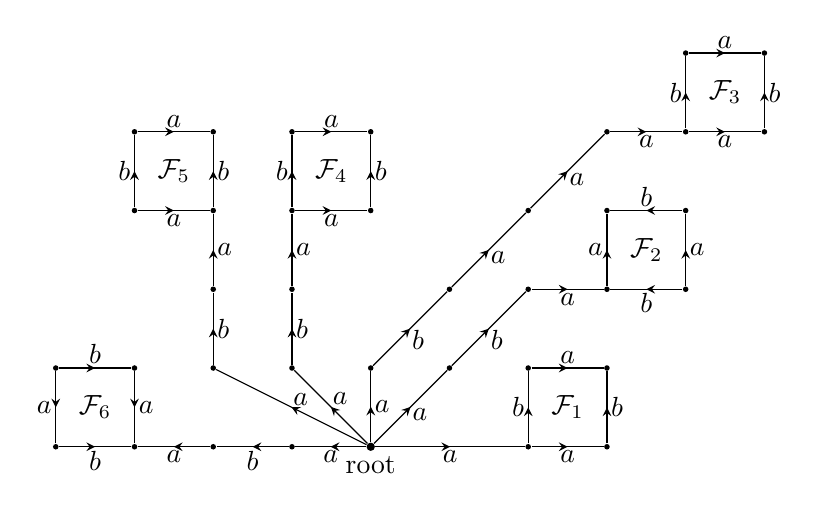
\begin{tikzpicture}[>=stealth,decoration={
				markings,
				mark=at position 0.5 with {\arrow{>}}}
	]

	\node[circle,fill=black,inner sep=0pt,minimum size=3pt] (root) at (0,0){} node[below]{root};
	\node[circle,fill=black,inner sep=0pt,minimum size=2pt] (n1) at (0,1) {};

	\draw[postaction={decorate}] (root) --node[right=-2pt]{$a$} (n1);

	\node[circle,fill=black,inner sep=0pt,minimum size=2pt] (m1) at (2,0) {};
	\node[circle,fill=black,inner sep=0pt,minimum size=2pt] (m2) at (3,0) {};
	\node[circle,fill=black,inner sep=0pt,minimum size=2pt] (m3) at (3,1) {};
	\node[circle,fill=black,inner sep=0pt,minimum size=2pt] (m4) at (2,1) {};

	\draw[postaction={decorate}] (root) --node[below=-2pt]{$a$} (m1);
	\draw[postaction={decorate}] (m1) --node[below=-2pt]{$a$} (m2);
	\draw[postaction={decorate}] (m2) --node[right=-2pt]{$b$} (m3);
	\draw[postaction={decorate}] (m1) --node[left=-2pt]{$b$} (m4);
	\draw[postaction={decorate}] (m4) --node[above=-2pt]{$a$} (m3);

	\node (f1) at (2.5,0.5) {$\mathcal F_1$};

	\node[circle,fill=black,inner sep=0pt,minimum size=2pt] (m5) at (1,1) {};
	\node[circle,fill=black,inner sep=0pt,minimum size=2pt] (m6) at (2,2) {};
	\node[circle,fill=black,inner sep=0pt,minimum size=2pt] (m7) at (3,2) {};
	\node[circle,fill=black,inner sep=0pt,minimum size=2pt] (m8) at (4,2) {};
	\node[circle,fill=black,inner sep=0pt,minimum size=2pt] (m9) at (4,3) {};
	\node[circle,fill=black,inner sep=0pt,minimum size=2pt] (m10) at (3,3) {};

	\draw[postaction={decorate}] (root) --node[below right=-4pt]{$a$} (m5);
	\draw[postaction={decorate}] (m5) --node[below right=-4pt]{$b$} (m6);
	\draw[postaction={decorate}] (m6) --node[below=-2pt]{$a$} (m7);
	\draw[postaction={decorate}] (m8) --node[below=-2pt]{$b$} (m7);
	\draw[postaction={decorate}] (m9) --node[above=-2pt]{$b$} (m10);
	\draw[postaction={decorate}] (m7) --node[left=-2pt]{$a$} (m10);
	\draw[postaction={decorate}] (m8) --node[right=-2pt]{$a$} (m9);

	\node (f2) at (3.5,2.5) {$\mathcal F_2$};
  
	\node[circle,fill=black,inner sep=0pt,minimum size=2pt] (m11) at (1,2) {};
	\node[circle,fill=black,inner sep=0pt,minimum size=2pt] (m12) at (2,3) {};
	\node[circle,fill=black,inner sep=0pt,minimum size=2pt] (m13) at (3,4) {};
	\node[circle,fill=black,inner sep=0pt,minimum size=2pt] (m14) at (4,4) {};
	\node[circle,fill=black,inner sep=0pt,minimum size=2pt] (m15) at (5,4) {};
	\node[circle,fill=black,inner sep=0pt,minimum size=2pt] (m16) at (5,5) {};
	\node[circle,fill=black,inner sep=0pt,minimum size=2pt] (m17) at (4,5) {};

	\draw[postaction={decorate}] (n1) --node[below right=-4pt]{$b$} (m11);
	\draw[postaction={decorate}] (m11) --node[below right=-4pt]{$a$} (m12);
	\draw[postaction={decorate}] (m12) --node[below right=-4pt]{$a$} (m13);
	\draw[postaction={decorate}] (m13) --node[below=-2pt]{$a$} (m14);
	\draw[postaction={decorate}] (m14) --node[below=-2pt]{$a$} (m15);
	\draw[postaction={decorate}] (m14) --node[left=-2pt]{$b$} (m17);
	\draw[postaction={decorate}] (m15) --node[right=-2pt]{$b$} (m16);
	\draw[postaction={decorate}] (m17) --node[above=-2pt]{$a$} (m16);

	\node (f3) at (4.5,4.5) {$\mathcal F_3$};

	\node[circle,fill=black,inner sep=0pt,minimum size=2pt] (m4_1) at (-1,1) {};
	\node[circle,fill=black,inner sep=0pt,minimum size=2pt] (m4_2) at (-1,2) {};
	\node[circle,fill=black,inner sep=0pt,minimum size=2pt] (m4_3) at (-1,3) {};
	\node[circle,fill=black,inner sep=0pt,minimum size=2pt] (m4_4) at (0,3) {};
	\node[circle,fill=black,inner sep=0pt,minimum size=2pt] (m4_5) at (0,4) {};
	\node[circle,fill=black,inner sep=0pt,minimum size=2pt] (m4_6) at (-1,4) {};

	\draw[postaction={decorate}] (root) --node[above right=-4pt]{$a$} (m4_1);
	\draw[postaction={decorate}] (m4_1) --node[right=-2pt]{$b$} (m4_2);
	\draw[postaction={decorate}] (m4_2) --node[right=-2pt]{$a$} (m4_3);
	\draw[postaction={decorate}] (m4_3) --node[below=-2pt]{$a$} (m4_4);
	\draw[postaction={decorate}] (m4_6) --node[above=-2pt]{$a$} (m4_5);
	\draw[postaction={decorate}] (m4_3) --node[left=-2pt]{$b$} (m4_6);
	\draw[postaction={decorate}] (m4_4) --node[right=-2pt]{$b$} (m4_5);

	\node (f4) at (-0.5,3.5) {$\mathcal F_4$};

	\node[circle,fill=black,inner sep=0pt,minimum size=2pt] (m5_1) at (-2,1) {};
	\node[circle,fill=black,inner sep=0pt,minimum size=2pt] (m5_2) at (-2,2) {};
	\node[circle,fill=black,inner sep=0pt,minimum size=2pt] (m5_3) at (-2,3) {};
	\node[circle,fill=black,inner sep=0pt,minimum size=2pt] (m5_4) at (-3,3) {};
	\node[circle,fill=black,inner sep=0pt,minimum size=2pt] (m5_5) at (-3,4) {};
	\node[circle,fill=black,inner sep=0pt,minimum size=2pt] (m5_6) at (-2,4) {};

	\draw[postaction={decorate}] (root) --node[above right=-4pt]{$a$} (m5_1);
	\draw[postaction={decorate}] (m5_1) --node[right=-2pt]{$b$} (m5_2);
	\draw[postaction={decorate}] (m5_2) --node[right=-2pt]{$a$} (m5_3);
	\draw[postaction={decorate}] (m5_4) --node[below=-2pt]{$a$} (m5_3);
	\draw[postaction={decorate}] (m5_5) --node[above=-2pt]{$a$} (m5_6);
	\draw[postaction={decorate}] (m5_3) --node[right=-2pt]{$b$} (m5_6);
	\draw[postaction={decorate}] (m5_4) --node[left=-2pt]{$b$} (m5_5);

	\node (f5) at (-2.5,3.5) {$\mathcal F_5$};

	\node[circle,fill=black,inner sep=0pt,minimum size=2pt] (m6_1) at (-1,0) {};
	\node[circle,fill=black,inner sep=0pt,minimum size=2pt] (m6_2) at (-2,0) {};
	\node[circle,fill=black,inner sep=0pt,minimum size=2pt] (m6_3) at (-3,0) {};
	\node[circle,fill=black,inner sep=0pt,minimum size=2pt] (m6_4) at (-3,1) {};
	\node[circle,fill=black,inner sep=0pt,minimum size=2pt] (m6_5) at (-4,1) {};
	\node[circle,fill=black,inner sep=0pt,minimum size=2pt] (m6_6) at (-4,0) {};

	\draw[postaction={decorate}] (root) --node[below=-2pt]{$a$} (m6_1);
	\draw[postaction={decorate}] (m6_1) --node[below=-2pt]{$b$} (m6_2);
	\draw[postaction={decorate}] (m6_2) --node[below=-2pt]{$a$} (m6_3);
	\draw[postaction={decorate}] (m6_4) --node[right=-2pt]{$a$} (m6_3);
	\draw[postaction={decorate}] (m6_5) --node[left=-2pt]{$a$} (m6_6);
	\draw[postaction={decorate}] (m6_6) --node[below=-2pt]{$b$} (m6_3);
	\draw[postaction={decorate}] (m6_5) --node[above=-2pt]{$b$} (m6_4);

	\node (f6) at (-3.5,0.5) {$\mathcal F_6$};


\end{tikzpicture}
\end{document}
